\documentclass[xcolor=dvipsnames,table]{beamer}

\usepackage{latexsym}
\usepackage[utf8]{inputenc}
\usepackage[brazil]{babel}
\usepackage{amssymb}
\usepackage{amsmath}
\usepackage{stmaryrd}
\usepackage{fancybox}
\usepackage{datetime}
\usepackage[T1]{fontenc}
\usepackage{graphicx}
\usepackage{graphics}
\usepackage{url}
\usepackage{algorithmic}
\usepackage{algorithm}
\usepackage{acronym}
\usepackage{array}

\newtheorem{definicao}{Definio}
\newcommand{\tab}{\hspace*{2em}}

\mode<presentation>
{
  \definecolor{colortexto}{RGB}{0,0,0}
 
  \setbeamertemplate{background canvas}[vertical shading][ bottom=white!10,top=white!10]
  \setbeamercolor{normal text}{fg=colortexto} 

  \usetheme{Warsaw}
}

\title{Terminologia de Descrição de MTs e Revisão} 

\author{
  Esdras Lins Bispo Jr. \\ \url{bispojr@ufg.br}
  } 
 \institute{
  Teoria da Computação \\Bacharelado em Ciência da Computação}
\date{\textbf{07 de dezembro de 2017} }

\logo{
\includegraphics[width=1cm]{images/ufgJataiLogo.png}}

\begin{document}

	\begin{frame}
		\titlepage
	\end{frame}

	\AtBeginSection{
		\begin{frame}{Sumário}%[allowframebreaks]{Sumário}
    		\tableofcontents[currentsection]
    		%\tableofcontents[currentsection, hideothersubsections]
		\end{frame}
	}

	\begin{frame}{Plano de Aula}
		\tableofcontents
		%\tableofcontents[hideallsubsections]
	\end{frame}
	
	
%------------------------------------------
	\section{Revisão}
	\subsection{Problemas Insolúveis em MT}
	
	\begin{frame}{Definição de Algoritmo}
		\begin{block}{Problema análogo}
			$D_1 = \{p \mbox{ | } p$ é um polinômio sobre $x$ com uma raiz inteira$\}$
		\end{block}  
		\begin{block}{MT $M_1$ que reconhece $D_1$}
			$M_1$ = ``A entrada é um polinômio $p$ sobre a variável $x$.
			\begin{enumerate}
				\item Calcule o valor de $p$ com $x$ substituída sucessivamente pelos valores $0, 1,-1, 2, -2, 3, -3, \ldots$ \\Se em algum ponto o valor do polinômio resulta em $0$, {\it aceite}.
			\end{enumerate}
		\end{block} 
		\begin{block}{Considerações}
			$M_1$ reconhece $D_1$, mas não a decide.
		\end{block}
	\end{frame} 
	
	\begin{frame}[shrink]{Definição de Algoritmo}
		\begin{block}{Resultado obtido por Matijasevich}
			É possível construir um decisor para $D_1$. Mas não para $D$.
		\end{block}  
		\begin{block}{Justificativa}
			É possível obter um limitante para polinômios de uma única variável. Porém, Matijasevich provou ser impossível calcular tais limitantes para polinômios multivariáveis.
		\end{block} 
		\begin{block}{Limitante para polinômios de uma única variável}
			\begin{center}
				$\pm k \dfrac{c_{max}}{c_1}$
			\end{center}
			em que 
			\begin{itemize}
				\item $k$ é o número de termos do polinômio,
				\item $c_{max}$ é o coeficiente com maior valor absoluto, e
				\item $c_1$ é o coeficiente do termo de mais alta ordem.
			\end{itemize}  
		\end{block}
	\end{frame}

	\subsection{Terminologia para descrever MTs}
	\begin{frame}{Terminologia para descrever MTs}
		\begin{block}{Níveis de descrição}
			\begin{itemize}
				\item {\bf Descrição formal}: esmiúça todos os elementos da 7-upla, conforme definição;
				\item {\bf Descrição de implementação}: descreve a forma pela qual a MT move a sua cabeça e a forma como ela armazena os dados na fita;
				\item {\bf Descrição de alto nível}: neste nível não precisamos mencionar como a máquina administra a sua fita ou sua cabeça de leitura-escrita.
			\end{itemize}
		\end{block}
	\end{frame}
	
	\section{Instrução pelos Colegas}
	\begin{frame}
		\begin{block}{Pergunta 1}
			Em relação à máquina de Turing, é {\bf incorreto} afirmar que...
		\end{block}
		\begin{enumerate}[(A)]
			\item Uma máquina de Turing pode tanto escrever sobre a fita quanto ler a partir dela.
			\item A cabeça de leitura–escrita pode mover-se tanto para a esquerda quanto para a direita.
			\item A fita é infinita.
			\item Os estados especiais para rejeitar e aceitar fazem efeito apenas após a leitura de toda a cadeia.
		\end{enumerate}
	\end{frame}

	\begin{frame}
		\begin{block}{Pergunta 2}
			O valor de retorno da função de transição $\delta$ de uma máquina de Turing é...
		\end{block}
		\begin{enumerate}[(A)]
			\item uma tripla contendo o estado de destino, o símbolo a ser escrito na fita e o movimento da cabeça.
			\item uma dupla contendo o símbolo a ser escrito na fita e o movimento da cabeça.
			\item uma tripla contendo o estado de origem, o símbolo a ser lido na fita e o movimento da cabeça.
			\item uma dupla contendo o símbolo a ser lido na fita e o movimento da cabeça.
		\end{enumerate}
	\end{frame}

	\begin{frame}
		\begin{block}{Pergunta 3}
			Sobre o alfabeto da fita $\Gamma$ e o alfabeto da linguagem $\Sigma$ é {\bf incorreto} afirmar que...
		\end{block}
		\begin{enumerate}[(A)]
			\item $\sqcup \in \Gamma$ 
			\item $\Gamma \subseteq \Sigma$
			\item $\Sigma \subseteq \Gamma$
			\item $\Sigma \subset \Gamma$
		\end{enumerate}
	\end{frame}

	\begin{frame}
		\begin{block}{Pergunta 4}
			Quantos estados, no mínimo, uma máquina de Turing pode ter?
		\end{block}
		\begin{enumerate}[(A)]
			\item um
			\item dois
			\item três
			\item nenhum
		\end{enumerate}
	\end{frame}

	\begin{frame}
		\begin{block}{Pergunta 5}
			Para se provar que a classe de linguagens decidíveis é fechada sob a operação de união, é necessário...
		\end{block}
		\begin{enumerate}[(A)]
			\item construir uma máquina de Turing que reconhece $A \cup B$, sendo $A$ e $B$ duas linguagens decidíveis quaisquer.
			\item construir a linguagem $A$ e a linguagem $B$, a partir de um decisor para $A \cup B$ qualquer.
			\item construir um decisor para $A \cup B$, sendo $A$ e $B$ duas linguagens decidíveis quaisquer.
			\item construir uma máquina de Turing que reconhece $A \cup B$, sendo $A$ e $B$ duas linguagens quaisquer.
		\end{enumerate}
	\end{frame}

	\begin{frame}
		\begin{block}{Pergunta 6}
			A classe de linguagens Turing-reconhecíveis {\bf não} é fechada sob a operação de complemento. Isto deve-se ao fato de...
		\end{block}
		\begin{enumerate}[(A)]
			\item uma máquina de Turing qualquer admitir a possibilidade de entrar em {\it loop} infinito.
			\item não termos conhecimento prévio sobre qual será a cadeia de entrada que será fornecida para a máquina.
			\item qualquer máquina de Turing ter uma fita infinita, não permitindo saber se a cadeia será aceita ou não pela máquina.
			\item termos que utilizar uma máquina de Turing de uma única fita (ao invés de uma multifita).
		\end{enumerate}
	\end{frame}

	\begin{frame}
		\begin{block}{Pergunta 7}
			O russo Yuri Matijasevic mostrou que era impossível conceber um algoritmo que testasse se um polinômio qualquer tem ou não raiz inteira. Em outros termos, ele provou que...
		\end{block}
		\begin{enumerate}[(A)]
			\item a linguagem associada a este problema não é Turing-reconhecível. 
			\item não existe uma máquina de Turing que reconheça a linguagem associada a este problema.
			\item não existe uma linguagem associada a este problema.
			\item não existe uma máquina de Turing que decida a linguagem associada a este problema.
		\end{enumerate}
	\end{frame}

	\begin{frame}
		\begin{block}{Pergunta 8}
			
			\begin{columns}
				\begin{column}{0.05\textwidth}\end{column}
				\begin{column}{0.45\textwidth}
					A maioria das estruturas de dados podem ser representadas por uma cadeia. Qual das alternativas {\bf não} é uma representação válida do grafo apresentado na figura ao lado?
				\end{column}
				\begin{column}{0.5\textwidth}  %%<--- here
					\begin{center}
						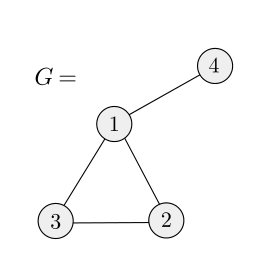
\includegraphics[width=.6\textwidth]{images/grafo}
					\end{center}
				\end{column}
			\end{columns}
			\begin{center}
				
			\end{center}
		\end{block}
		\begin{enumerate}[(A)]
			\item (1,2,3,4)((1,2),(2,3),(3,1),(1,4)) 
			\item (1\#2, 2\#3, 3\#1, 1\#4)
			\item 12, 23, 31, 14 / 1-3-4
			\item 12 - 23 - 31 - 14
		\end{enumerate}
	\end{frame}
	
	\begin{frame}
		\titlepage
	\end{frame}
	
\end{document}